\documentclass[]{article}
\usepackage{lmodern}
\usepackage{amssymb,amsmath}
\usepackage{ifxetex,ifluatex}
\usepackage{fixltx2e} % provides \textsubscript
\ifnum 0\ifxetex 1\fi\ifluatex 1\fi=0 % if pdftex
  \usepackage[T1]{fontenc}
  \usepackage[utf8]{inputenc}
\else % if luatex or xelatex
  \ifxetex
    \usepackage{mathspec}
  \else
    \usepackage{fontspec}
  \fi
  \defaultfontfeatures{Ligatures=TeX,Scale=MatchLowercase}
\fi
% use upquote if available, for straight quotes in verbatim environments
\IfFileExists{upquote.sty}{\usepackage{upquote}}{}
% use microtype if available
\IfFileExists{microtype.sty}{%
\usepackage{microtype}
\UseMicrotypeSet[protrusion]{basicmath} % disable protrusion for tt fonts
}{}
\usepackage[margin=1in]{geometry}
\usepackage{hyperref}
\PassOptionsToPackage{usenames,dvipsnames}{color} % color is loaded by hyperref
\hypersetup{unicode=true,
            colorlinks=true,
            linkcolor=Maroon,
            citecolor=Blue,
            urlcolor=blue,
            breaklinks=true}
\urlstyle{same}  % don't use monospace font for urls
\usepackage{graphicx,grffile}
\makeatletter
\def\maxwidth{\ifdim\Gin@nat@width>\linewidth\linewidth\else\Gin@nat@width\fi}
\def\maxheight{\ifdim\Gin@nat@height>\textheight\textheight\else\Gin@nat@height\fi}
\makeatother
% Scale images if necessary, so that they will not overflow the page
% margins by default, and it is still possible to overwrite the defaults
% using explicit options in \includegraphics[width, height, ...]{}
\setkeys{Gin}{width=\maxwidth,height=\maxheight,keepaspectratio}
\IfFileExists{parskip.sty}{%
\usepackage{parskip}
}{% else
\setlength{\parindent}{0pt}
\setlength{\parskip}{6pt plus 2pt minus 1pt}
}
\setlength{\emergencystretch}{3em}  % prevent overfull lines
\providecommand{\tightlist}{%
  \setlength{\itemsep}{0pt}\setlength{\parskip}{0pt}}
\setcounter{secnumdepth}{0}
% Redefines (sub)paragraphs to behave more like sections
\ifx\paragraph\undefined\else
\let\oldparagraph\paragraph
\renewcommand{\paragraph}[1]{\oldparagraph{#1}\mbox{}}
\fi
\ifx\subparagraph\undefined\else
\let\oldsubparagraph\subparagraph
\renewcommand{\subparagraph}[1]{\oldsubparagraph{#1}\mbox{}}
\fi

%%% Use protect on footnotes to avoid problems with footnotes in titles
\let\rmarkdownfootnote\footnote%
\def\footnote{\protect\rmarkdownfootnote}

%%% Change title format to be more compact
\usepackage{titling}

% Create subtitle command for use in maketitle
\newcommand{\subtitle}[1]{
  \posttitle{
    \begin{center}\large#1\end{center}
    }
}

\setlength{\droptitle}{-2em}
  \title{}
  \pretitle{\vspace{\droptitle}}
  \posttitle{}
  \author{}
  \preauthor{}\postauthor{}
  \date{}
  \predate{}\postdate{}

\usepackage{fancyhdr}
\pagestyle{fancy}
\fancyhead[RE,RO]{Andreas Havmøller Johnsen}
\fancyhead[LE,LO]{Medialogy, CPH, 2017}
\fancyfoot[CE,CO]{STUDY VERIFICATION TEST}
\fancyfoot[LE,RO]{\thepage}

\begin{document}

\section{Study Verification Test - Student
Report}\label{study-verification-test---student-report}

This is an interpretive report of your responses to the study
verification test. Its purpose is to help you identify your student
profile within specific topics.

The boxplots\footnote{A \emph{boxplot} consists of four equal sized
  groups made from the ordered scores, i.e.~25\% of all scores are
  placed in each group. The lines dividing the groups are called
  quartiles. The rectangular box denotes the middle 50\% of scores for
  the group, and its lengyh is equal to the difference between the 75th
  and 25th percentiles. The median (middle quartile) marks the mid-point
  of the data, indicated as the line dividing the box into two parts.
  The upper and lower lines (also called whiskers) represent scores
  outside the middle 50\%. Outliers are defined as data points outside
  the whiskers and plotted as black dots.} show how you compare to a
larger sample of first semester Medialogy students from Aalborg and
Copenhagen. Specifically, they indicate the average self-ratings of all
students in seven different topics (see Figure 1) and the self-reported
study hours per week (see Figure 2). Your self-reported value for each
topic is indicated with red dots. A value less than 0.5 means that you
rated yourself lower than the average student. The percentiles indicate
the percentage of students whose scores are equal to or less than yours.
Based on these results we have created specific recommendations for you
to get more comfortable in the Medialogy study environment.

As the report is based on the questionnaire information alone, it may
give only a rough indication of your true attitudes. Your advisor or
student counselor will help you understand your scores and find the
services you desire.

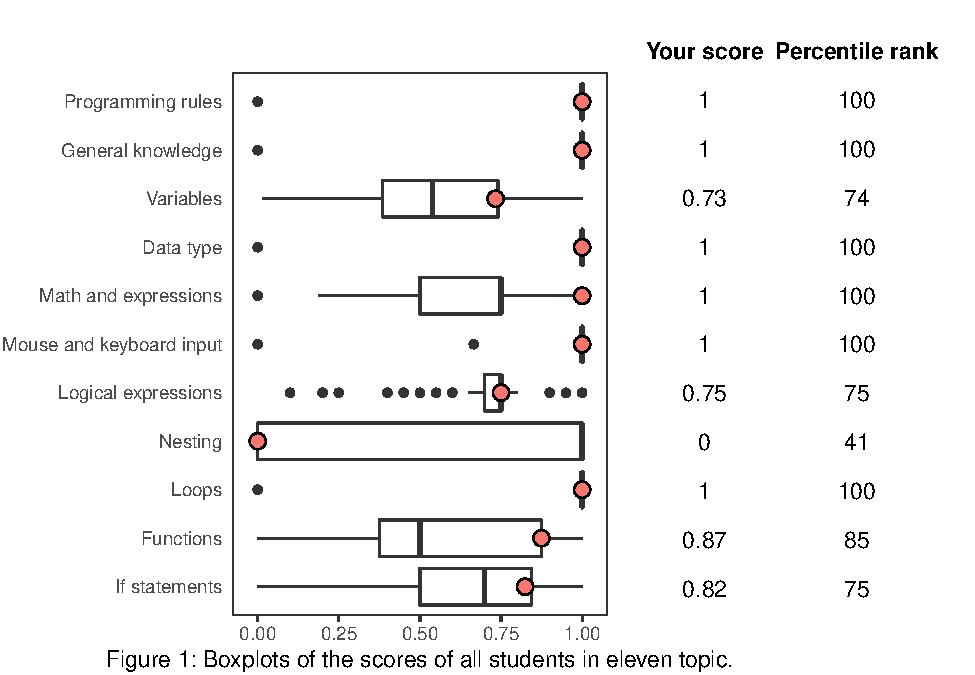
\includegraphics{C:/Users/BiancaClavio/Documents/stats-on-grades/docs/handouts/SSPanalysis_1_files/figure-latex/unnamed-chunk-4-1.pdf}

\includegraphics{C:/Users/BiancaClavio/Documents/stats-on-grades/docs/handouts/SSPanalysis_1_files/figure-latex/unnamed-chunk-5-1.pdf}

\pagebreak

\subsection{Specific Recommondations}\label{specific-recommondations}

In this section you will receive a more detailed explanation of your
results. The purpose of this information is to help you develop your
skills and get the most from your university experience. Take a balanced
approach to reviewing and utilizing this information. Do not assume that
each statement is perfectly accurate just because it is printed in a
formal manner; some statements may not fit you well. However, do not
dismiss a statement just because it points to a challenge.

Keep an open mind as you consider each statement. When it seems
accurate, give serious thought to any suggestions that accompany the
statement. If the statement is puzzling, discuss it with someone who can
help you interpret it. Approaching the information in this way can be
very helpful.

\paragraph{Social Support for
Studying}\label{social-support-for-studying}

Studying is a long-term endeavour and there will be times of frustration
and doubt. Your self-reported social support for studying placed you in
the 27th percentile, and your responses suggest that you enrolled for a
university degree in general and Medialogy at AAU specifically without
having received a large amount of encouragement from friends, family, or
other sources. During your education it can help to have a social
network that understands that times of frustration can be part of
pursuing a higher education degree. Your social network can support you
in times of hardship, doubt, and low morale. It is good to hear that you
have already made some friends at AAU. Making friends with fellow
students at university can be a valuable source to rely on throughout
the education. Taking active part in student unions, being a volunteer
at events, or other types of student environment activities can help
you. It will broaden your social reference beyond your own semester or
education. Breaking the barrier to seek social network outside your own
semester can seem daunting, but can become a significantly positive part
of your years as university student. If in doubt about how to initiate
or engage, consider having a chat with your student counselor.

\paragraph{High School Habits}\label{high-school-habits}

In high school, the teacher often has the responsibility of giving
homework, communicating learning material, recording attendance in
class, ensure student progress, and help the students when required.
Your self-reported high school habits placed you in the 15th percentile,
which suggests that you As a student at university, you have the
responsibility for what you learn. Your lecturers will often have more
focus on academic content than on pedagogy, and weak study habits can
therefore set you back in your learning progress and potential. can
majorly benefit from reflecting on your study habits. A personal
reflection on how you may need to change your habits for university, can
result in more efficient work, a much better study life experience, and
a much higher quality skillset. Remember, when you graduate after three
or five years of studies, you need to have placed sufficient effort,
gained sufficient experience and acquired sufficient knowledge, to be
confident in your abilities. If your habits keep you from reaching your
potential, you might not have the credentials for field-relevant or
interesting jobs. You will then have lost 5 years of your potential,
that you will not get back. Ergo; start visualizing the prospects you
believe your education should provide you, by the end of your student
journey. Use the propects in order to fuel your habit change, direct
your ambition, as well as your sense of personal responsibility for your
future.

\paragraph{Study Habits}\label{study-habits}

Weak study habits are the single greatest cause of academic problems at
university. Your self-reported study habits placed you in the 34th
percentile, and you will benefit from adopting more good study habits.
As soon as possible, develop a clear daily routine in which you set
aside certain periods of time to study. Learn to focus your attention
and to pace yourself. Find the situations or circumstances, where your
attention is challenged or removed from otherwise study-allocated time
or activity. Examples can be when sitting too far back in the room
during the lectures while keeping focused attention, or when
multitasking too many activities while keeping the mind from wandering
away from the subject matter during homework sessions. Other useful
techniques include previewing, underlining, note-taking, and reviewing.
Academic counselors can help you develop your study habits and exercises
for keeping focus. You can find a set of helpful tools to improve your
study habits \href{tinyurl.com/AAUstudyPlanning}{here}
(tinyurl.com/AAUstudyPlanning) and find study related exercises
\href{tinyurl.com/AAUstudySkillsExercises}{here}
(tinyurl.com/AAUstudySkillsExercises).

\paragraph{Grit}\label{grit}

Talent without hard work rarely amounts to anything ambitious. Making
the effort to stay with a problem (or challenge) for long enough,
increases your chances of cracking it and mastering new skills. This
requires time and dedication, and is known as grit. Students with high
self-reported values in grit, are less likely to drop out and fail exams
than those with lower scores. Your self-reported grit places you in the
27th percentile, and it appears you would benefit from more perseverance
and dedication to solving problems, achieving study goals, etc. Previous
Medialogy cohorts have shown that no matter the high school diploma,
students can make it through the education if they persist, and invest
the time and effort. Grit is a part of university life. Despite being a
demanding part, it is often also what leads to rewarding experiences and
new skill sets. Remember this next time you encounter a difficult
problem and you feel like giving up. Remove yourself from distractions,
be tenacious, and keep grinding.

\paragraph{Growth mindset}\label{growth-mindset}

Seeing your intelligence as something that you can actively influence
and grow is referred to as having a growth mindset. Students with high
self-reported values in growth mindset are less likely to drop out and
fail exams than those with lower scores. Your self-reported
understanding of intelligence placed you in the 59th percentile, meaning
that you are open to actively improving your intelligence. Seeing
setbacks (failed assignments or poor exam grades) as an opportunity to
learn and grow rather than inadequacy, lack of intelligence or talent
helps you overcome challenges and develop a positive learning attitude.

\paragraph{Study and Work}\label{study-and-work}

Studying requires a lot of time and dedication in order to succeed.
Being intelligent and having talent can help but does not replace the
need for dedicating time and effort to studying. The ECTS system assumes
that you spend 45 hours a week on your education. You reported using 55
hours weekly for studying, which indicates that you are using less than
the recommended amount of time for studying. Meeting these demands is
difficult over long-term with too many other obligations. You reported
using 0 hours on study related work, and 10 hours on non-study related
work. Should you not able to dedicate around 45 hours to study each
week, you should not despair when you fail exams. You simply did not
have the time resources to succeed and studying might take longer than
expected. However, if you mainly rely on SU this provides a clear time
frame within which you need to finish your education. You should
therefore carefully review your commitments and other activities that
you need or want to dedicate time to vis-à-vis the study demands.

\paragraph{Understanding of Medialogy}\label{understanding-of-medialogy}

Choosing a suitable education can be difficult, and students should
reflect on their choice of education, especially, in the first
semester(s). Your understanding about what you will learn in the
Medialogy programme is in the 14th percentile, meaning that your
understanding of Medialogy is rather different from what the study plan
indicates. Medialogy has a strong technical foundation but offers many
other skills and competencies that give you opportunities to design
novel technologies and this usually involves programming. Contrary to
what you indicated in the study verification questionnaire Medialogy
students learn only little about: manual content creation, work with
aesthetics, professional moving making, and working as a rigging artist
Although you have group responsibilities related to you project, the
group is not responsible of the individual learning goals, defined in
the study plan. Previous students with different expectations either
learned to appreciate the content, skills, and opportunities of a
Medialogy degree or changed to other programmes or educations. Attending
the Med Awards event (usually in November) and seeing other student
projects can give you an idea of what you will be able to do if you
apply yourself to what Medialogy can offer. Contacting older students in
the Medialogy facebook group, study counselors, and going to the study
cafe can also provide you information about the education and what it
means to be a Medialogy student. You can find information about
Medialogy and student testimonials
\href{tinyurl.com/AAUaboutMedialogy}{here}
(tinyurl.com/AAUaboutMedialogy).


\end{document}
